\section{Hybrid Techniques}
So far we have discovered Graph-based solutions, using close proximity devices, such as RFID, NFC, and Bluetooth and Fingerprinting techniques using Wi-Fi. 
Combining the Wi-Fi based fingerprinting with low proximity technology such as Bluetooth has been done with good results~\cite{6068444}.
As mentioned in Section~\ref{wififingerprinting} Wi-Fi solutions have several issues regarding accuracy, but it has low infrastructure cost -- as it is often already deployed -- and high range. 
Bluetooth technology is quite the opposite as it is rarely deployed in buildings, it has a short range. 
The short range ensure that positions can be estimated fairly accurately as whenever a device can read the signal from a Bluetooth transmitter it is physically located close to transmitter. 
Bluetooth transmitters have varying propagation distances, but it is preferred for the technique explained in the following that the range is short. 
The technique which we have investigated are described in~\cite{6068444}.

%\subsection{Basic Concept}  
The idea is to partition the indoor space into regions using Bluetooth transmitters.
An example of such an partition is shown in Figure \ref{fig:partionedcluster}. 
Here position 5, 7, and, 19 contains a Bluetooth transmitter that the user cannot pass without the device he uses for position determination registers the sender.  
%The cluster in Figure \ref{fig:partionedcluster} contains 4 regions. 

\begin{figure}%
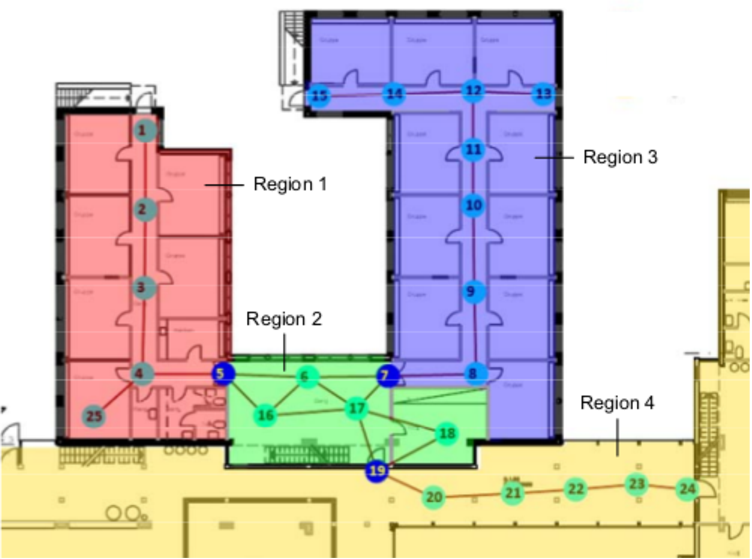
\includegraphics[width=\columnwidth]{images/partionedcluster}%
\caption{An indoor space partitioned into four region. Adapted from~\cite{6068444}.}%
\label{fig:partionedcluster}%j
\end{figure}%   
The partitioning is done at narrow places, such as hallways and doorways. 
This is necessary to ensure that a user cannot pass through the Bluetooth transmitter without noticing it. 
Once a user passes a Bluetooth transmitter in an indoor space we can limit his possible position to two regions. 
E.g. if a user is registered at the transmitter in location 7 in Figure \ref{fig:partionedcluster} he can be in either region 2 or 3. 
Until the user passes another Bluetooth transmitter he can be assumed to be in these two regions.
If he for instances passes the transmitter in location 5, he can be in either region 1 or 2. 
It is, however, not possible to determine the moving direction of the sender because he may have entered the proximity of the transmitter and then returned from where he came. 

%\subsection{Device and Architecture}
%The device is typically a smartphone (during the testing a small laptop is used) or similar with an application installed. 
%The application registers the Bluetooth and Wi-Fi signals strengths with $1/3$Hz and $1$Hz respectively.  
%The signal strengths are send to a server which calculates the position of the device. 
%The entire system architecture can be seen in Figure~\ref{fig:hybridsystemarchitecture}.
\begin{figure}%
    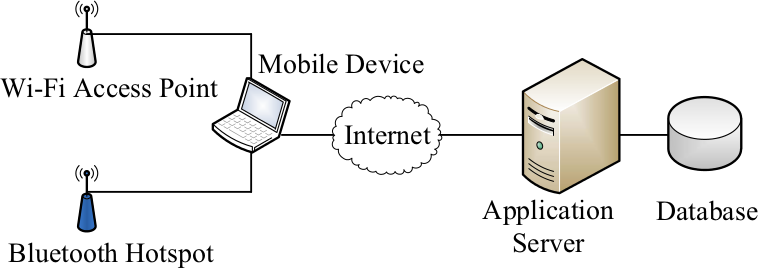
\includegraphics[width=\columnwidth]{images/hybridsystemarchitecture.png}%
\caption{The system architecture of the hybrid system. Adapted from~\cite{6068444}.}%
\label{fig:hybridsystemarchitecture}%
\end{figure}
%\subsection{Results}
From the test performed by the research team the hybrid technique improves the overall accuracy compared to purely Wi-Fi based techniques. 
Figure \ref{fig:hybridsystemarchitecture} shows the architecture of the tested system.
%Due to the partitioning of the indoor space, the search area for a query is very limited.
%Thus making each query perform relatively fast. %In~\cite{
  
